% !TeX spellcheck = cs_CZ
%{\tikzset{external/prefix={tikz/FYZII/}}
% \tikzset{external/figure name/.add={ch10_}{}}
%---------------------------------------------------------------------------------------------------
% file fey2ch10.tex
%---------------------------------------------------------------------------------------------------
%=========================== Kapitola: Dielektrika =================================================
\setchaptertoc
\chapter{Dielektrika}\label{fyz:IIchapX}
  \section{Permitivita}\label{fyz:IIchapXsecI}
    Na tomto místě začneme hovořit o další z charakteristických vlastností látky nacházející se pod
    vlivem elektrického pole. V jedné z předcházejících kapitol jsme se zabývali vlastnostmi
    \emph{vodičů}, v nichž se účinkem elektrického pole náboje volně přemisťují do takových míst, že
    uvnitř vodiče nezůstane žádné pole. Nyní budeme hovořit o \emph{izolantech}, tedy o látkách,
    které elektřinu nevedou. Na první pohled by se mohlo zdát, že se s nimi v elektrickém poli
    nestane vůbec nic. Ale Faraday pomocí jednoduchého elektroskopu a deskového kondenzátoru
    objevil, že tomu tak není. Jeho pokusy ukázaly, že kapacita takového kondenzátoru
    \emph{vzroste}, když se mezi jeho elektrody vloží izolant. Vyplní-li izolant prostor mezi
    elektrodami, kapacita se zvětší \(\varepsilon_r\)-krát, přičemž koeficient \(\varepsilon_r\)
    závisí pouze na vlastnostech izolační látky. Izolační látky se také nazývají \emph{dielektrika};
    součinitel \(\varepsilon_r\) je tedy vlastností dielektrika a nazývá se \emph{relativní
    permitivita}. Relativní permitivita vakua je, samozřejmě, rovna jedné.  

    Naší úlohou je nyní vysvětlit, proč vůbec nějaký elektrický efekt nastává, jsou-li izolanty
    opravdu izolanty a elektřinu nevedou. Vyjdeme z experimentálního faktu, že kapacita vzrůstá a
    pokusíme se vymyslet, co by se přitom mohlo dít. Uvažujme deskový kondenzátor s nějakými náboji
    na povrchu vodičů, řekněme se záporným nábojem na horní a s kladným nábojem na dolní elektrodě.
    Předpokládejme, že vzdálenost mezi elektrodami je \(d\) a plošný obsah každé elektrody je \(S\).
    Jak jsme viděli už dříve, kapacita kondenzátoru je
    \begin{equation}\label{fyz:eq907}
      C = \dfrac{\varepsilon_0S}{d}
    \end{equation}
    a náboj souvisí s napětím na kondenzátoru podle vztahu
    \begin{equation}\label{fyz:eq908}
      Q = CU.
    \end{equation}

    Experimentálním faktem je, že vložíme-li mezi desky kus izolantu, například skla nebo plexiskla,
    zjistíme, že se kapacita zvětší. To ovšem znamená, že při témže náboji se napětí snížilo. Ale
    napětí je integrálem elektrického pole počítaným napříč kondenzátorem; musíme tedy udělat závěr,
    že uvnitř kondenzátoru se zeslabilo elektrické pole, i když náboje na deskách zůstávají
    nezměněny.

    \begin{figure}[ht!] %\ref{fyz:fig705}
      \centering
      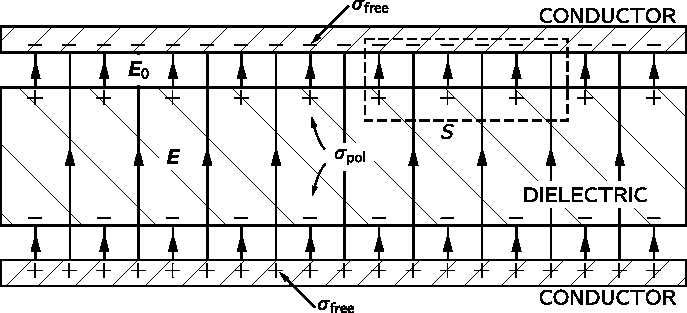
\includegraphics[width=0.9\linewidth]{fyz_fig705.pdf}
      \caption{Deskový kondenzátor s dielektrikem. Vyznačeny jsou siločáry elektrického pole \(E\).
               (\cite[s.~175]{Feynman02})}
      \label{fyz:fig705}
    \end{figure}

    Jak je to možné? Máme větu, pocházející od Gausse, která nám říká, že tok elektrického pole
    uzavřenou plochou je v přímém vztahu s náboji uvnitř plochy. Uvažujme gaussovskou plochu \(S\)
    vyznačenou na obr. \ref{fyz:fig705} čárkovaně. Protože elektrické pole se v přítomnosti
    dielektrika zeslabilo, usuzujeme, že celkový náboj uvnitř plochy musí být menší, než byl bez
    látky. Pak existuje jediný možný závěr a ten je, že na povrchu dielektrika musí sídlit kladné
    náboje. Protože se sice pole zeslabilo, ale ne na nulu, očekáváme, že tento kladný náboj je
    menší než záporný náboj na vodiči. Celý úkaz by bylo možné vysvětlit, kdybychom nějak uměli
    pochopit, proč se při umístění dielektrické látky do elektrického pole na jednom povrchu
    indukuje kladný a na druhém záporný náboj.

    Něco takového bychom očekávali v případě vodiče. Mějme například kondenzátor se vzdáleností
    \(d\) mezi elektrodami a vložme mezi ně neutrální vodič, jehož tloušťka je \(b\) (obr.
    \ref{fyz:fig706}). Elektrické pole indukuje kladný náboj na jeho horním povrchu a záporný náboj
    na jeho dolním povrchu, takže uvnitř vodiče pole není. Ve zbývajícím prostoru je pole totéž,
    jako by bylo bez vodiče, neboť je rovno plošné hustotě náboje dělené \(\varepsilon_0\) ale
    vzdálenost, přes kterou musíme integrovat, abychom dostali napětí (rozdíl potenciálů), se
    zmenšila.

    Napětí je
    \begin{equation*}
      U = \dfrac{U}{\varepsilon_0}(d-b).
    \end{equation*}
    Výsledný výraz pro kapacitu je stejný jako (\ref{fyz:eq907}), ale \(d\) je nahrazeno rozdílem
    \((d - b)\)
    \begin{equation}\label{fyz:eq909}
      C = \dfrac{\varepsilon_0S}{d\left[1 - (b/d)\right]}
    \end{equation}
    Kapacita se zvětšila v poměru, jenž závisí na \((b/d)\), tj. na poměrné části objemu, kterou
    zaujal vodič.

    \begin{figure}[ht!] %\ref{fyz:fig706}
      \centering
      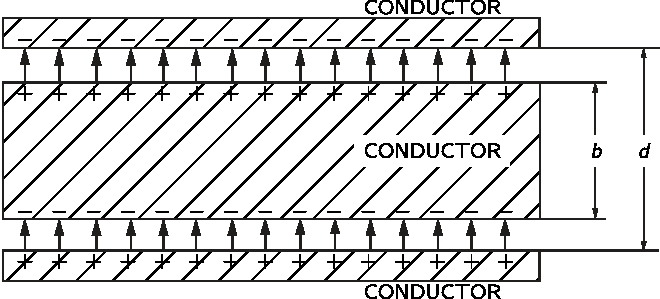
\includegraphics[width=0.9\linewidth]{fyz_fig706.pdf}
      \caption{Vložíme-li mezi elektrody deskového kondenzátoru vodivou desku, indukované náboje
               zeslabí pole uvnitř vodiče na nulovou hodnotu. (\cite[s.~175]{Feynman02})}
      \label{fyz:fig706}
    \end{figure}

    To nám však poskytuje zřejmý model toho, co se děje s dielektriky - uvnitř látky se nachází
    množství tenkých vodivých vrstev. S takovým modelem je však spojena jedna obtíž - má významnou
    osu, normálu k vrstvám, zatímco většina dielektrik takovou osu nemá. Ale tuto obtíž je možno
    vyloučit, uděláme-li předpoklad, že všechny izolační látky obsahují malé navzájem izolované
    vodivé koule, jak ukazuje obr. \ref{fyz:fig707}. Permitivita je vysvětlována působením nábojů,
    které by byly indukovány na každé kuličce. Je to jeden z prvních fyzikálních modelů dielektrika,
    použitých na vysvětlení jevu pozorovaného Faradayem. Konkrétněji řečeno, předpokládalo se, že
    každý z atomů látky je dokonalým vodičem, ale izolovaným od jiných atomů. Relativní permitivita
    \(\varepsilon_0\) bude záviset na tom, jakou část objemu zabírají vodivé koule. Dnes však tento
    model nepoužíváme.

    \begin{figure}[ht!] %\ref{fyz:fig707}
      \centering
      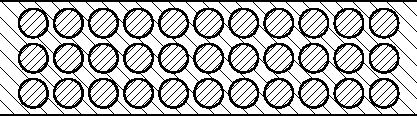
\includegraphics[width=0.9\linewidth]{fyz_fig707.pdf}
      \caption{Model dielektrika: malé vodivé kuličky zapuštěné do idealizovaného izolátoru
               (\cite[s.~176]{Feynman02})}
      \label{fyz:fig707}
    \end{figure}

  \section{Vektor elektrické polarizace P}\label{fyz:IIchapXsecII} 
    Pokračujeme-li v naší analýze, přijdeme na to, že představa o oblastech s dokonalou vodivostí a
    izolací mezi nimi není podstatná. Každá z malých kuliček se chová jako dipól, jehož moment je
    indukován vnějším polem. Jediná věc, jež je pro pochopení dielektrik podstatná je ta, že v
    dielektrické látce je indukováno mnoho malých dipólů. To, zda se dipóly indukují proto, že
    existují vodivé malé kuličky, nebo z nějakého jiného důvodu, je bezvýznamné.

    Proč by pole mělo v atomu indukovat dipólový moment, není-li atom vodivou koulí? O této otázce
    budeme mluvit mnohem podrobněji v následující kapitole, která bude věnována vnitřním procesům v
    dielektrických látkách. Zde však uvedeme jeden příklad, abychom ilustrovali možný mechanizmus.
    Kladný náboj atomu je v jádře, jež je obklopeno zápornými elektrony. Orbity nebo vlnové balíky
    elektronů (nebo jakékoliv zobrazení použité v kvantové mechanice) jsou v nějaké míře pokřiveny
    (obr. \ref{fyz:fig708}); těžiště záporného náboje se posune a nebude už splývat s kladným
    nábojem jádra. My jsme už o takovém rozdělení náboje hovořili. Díváme-li se na něj z velké
    vzdálenosti, je taková neutrální konfigurace v prvním přiblížení ekvivalentní malému dipólu.

    \begin{figure}[ht!]
      \centering
      \subcaptionbox{\label{fyz:fig708a}}{\luafigure[0.45]{fyz_fig708a.pdf}}
      \subcaptionbox{\label{fyz:fig708b}}{\luafigure[0.45]{fyz_fig708b.pdf}}
      \caption{Rozdělení elektronů v atomu nacházejícím se v elektrickém poli se vzhledem k jádru
              posune. (\cite[s.~177]{Feynman02})}
      \label{fyz:fig708}
    \end{figure}

    Asi je rozumné předpokládat, že není-li pole příliš silné, velikost indukovaného dipólového
    momentu bude přímo úměrná poli. Slabé pole tedy posune náboje jen o malý kousíček, zatímco silné
    pole je posune víc, a to přímo úměrně poli, jen když posunutí nebude příliš velké. Do konce této
    kapitoly budeme dipólový moment považovat za přesně přímo úměrný poli.

    Dále budeme předpokládat, že v každém atomu jsou náboje \(q\) ve vzájemné vzdálenosti
    \(\vec{δ}\) takže \(q\vec{δ}\) je elektrický dipólový moment připadající na jeden atom.
    (\(\vec{δ}\) používáme proto, neboť \(d\) jsme už použili pro vzdálenost elektrod.) Je-li v
    jednotkovém objemu \(N\) atomů, bude \textbf{dipólový moment jednotkového objemu} roven
    \(Nq\vec{δ}\). Tento elektrický dipólový moment připadající na jednotkový objem budeme označovat
    vektorem \(\vec{P}\). Není třeba zdůrazňovat, že leží ve směru jednotlivých dipólových momentů,
    tj. ve směru posunutí nábojů \(\vec{δ}\).
    \begin{equation}\label{fyz:eq910}
      \vec{P} = Nq\vec{δ}
    \end{equation}

    Obecně se bude \(\vec{P}\) v dielektriku měnit od místa k místu. Ale v každém bodě látky je
    přímo úměrné elektrickému poli. Součinitel této úměrnosti je určen tím, jak snadno se elektron
    posune, a závisí na druhu atomů v látce.
    
    O tom, co doopravdy určuje, jak se tento součinitel chová, jak přesně konstantní je ve velmi
    silných polích a co se děje uvnitř různých látek, budeme mluvit později. V této chvíli budeme
    prostě předpokládat, že existuje mechanizmus, jímž se indukuje elektrický dipólový moment přímo
    úměrný elektrickému poli.

  \section{Polarizační náboje}\label{fyz:IIchapXsecIII}   
    Nyní prozkoumejme, co z tohoto modelu vyplývá pro teorii kondenzátoru vyplněného dielektrikem.
    Nejdříve uvažujeme destičku z látky, která má určitý elektrický dipólový moment připadající na
    jednotkový objem. Vznikne v důsledku toho v průměru nějaká hustota náboje v látce? Ne, je-li
    \(\vec{P}\) homogenní. Mají-li kladné a záporné náboje po posunutí stejné hustoty náboje, z
    jejich posunutí nevzniká v objemu žádný výsledný náboj. Na druhé straně, kdyby \(\vec{P}\) bylo
    v jednom místě větší a v druhém místě menší, znamenalo by to, že se do některé oblasti přesunulo
    více náboje, než se z ní vysunulo ven; tehdy bychom mohli očekávat nenulovou objemovou hustotu
    náboje. V případě deskového kondenzátoru předpokládáme, že \(\vec{P}\) je homogenní, takže je
    nutné prozkoumat pouze to, co se děje na povrchu. Na jednom povrchu se záporné náboje -
    elektrony efektivně vysunuly do vzdálenosti \(δ\), zatímco na druhém povrchu se posunuly dovnitř
    a zanechaly určitý kladný náboj na vzdálenosti \(δ\). Jak ukazuje obr. \ref{fyz:fig709}, na
    povrchu vznikne plošná hustota náboje, který budeme nazývat \textbf{povrchovým polarizačním
    nábojem}.

    Tento náboj je možné vypočítat následujícím způsobem. Počet elektronů, které se objeví na
    povrchu destičky je roven součinu jejího plošného obsahu \(S\), počtu elektronů v jednotkovém
    objemu \(N\) a posunutí \(δ\), o němž zde předpokládáme, že nastane kolmo k povrchu. Výsledný
    náboj dostaneme vynásobením této hodnoty nábojem elektronu \(q_e\). Abychom dostali plošnou
    hustotu polarizačního náboje indukovaného na povrchu, musíme výsledek dělit plošným obsahem
    \(S\). Velikost plošné hustoty náboje tedy bude
    \begin{equation*}
      σ_{\text{pol}}=Nq_eδ.
    \end{equation*}
    To je však právě rovno velikosti \(P\) vektoru elektrické polarizace \(\vec{P}\), daného vztahem
    (\ref{fyz:eq910}), tj. 
    \begin{equation}\label{fyz:eq911}
      σ_{\text{pol}} = P.
    \end{equation}
    \emph{Plošná hustota náboje na povrchu látky je rovna elektrické polarizaci v jejím vnitřku.}
    Povrchový náboj je samozřejmě kladný na jedné straně a záporný na opačné straně povrchu.

    \begin{figure}[ht!] %\ref{fyz:fig709}
      \centering
      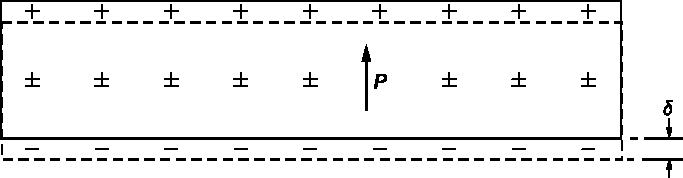
\includegraphics[width=1\linewidth]{fyz_fig709.pdf}
      \caption{Dielektrická vrstva v homogenním poli. Kladné náboje jsou posunuty do vzdálenosti
              \(δ\) vzhledem k záporným. (\cite[s.~177]{Feynman02})}
      \label{fyz:fig709}
    \end{figure}
    
    Dále předpokládejme, že naše deska představuje dielektrikum v rovinném kondenzátoru. Na
    \emph{elektrodách} kondenzátoru se také nachází plošný náboj, jehož hustotu označíme
    \(σ_{\text{free}}\), neboť ve vodiči se náboje mohou „volně“ pohybovat. Jde, samozřejmě, o
    náboj, který jsme dodali při nabíjení kondenzátoru. Je nutné zdůraznit, že \(σ_{\text{pol}}\)
    existuje jen proto, že existuje \(σ_{\text{free}}\). Odstraní-li se vybitím kondenzátoru
    \(σ_{\text{free}}\), vymizí také \(σ_{\text{pol}}\). Neodejde však vodičem, kterým se vybije
    kondenzátor, ale pohybem zpět dovnitř látky, a to rozptýlením polarizace uvnitř látky.

    Nyní můžeme na gaussovskou plochu \(S\), znázorněnou na obr. \ref{fyz:fig705}, použít Gaussův
    zákon. Elektrické pole \(\vec{E}\) v dielektriku je rovno celkové plošné hustotě náboje dělené
    \(\varepsilon_0\). Je zřejmé, že \(σ_{\text{pol}}\) a \(σ_{\text{free}}\) mají opačná znaménka,
    takže
    \begin{equation}\label{fyz:eq912}
      E = \dfrac{σ_{\text{free}} - σ_{\text{pol}}}{\varepsilon_0}.
    \end{equation}

    Všimněme si, že pole \(E_0\) mezi kovovou elektrodou a povrchem dielektrika je větší než pole
    \(E\); odpovídá pouze hustotě \(σ_{\text{free}}\). Zde se však zajímáme o pole uvnitř
    dielektrika. Vyplňuje-li dielektrikum téměř celou mezeru mezi elektrodami, je toto pole
    rozprostřeno prakticky v celém objemu uvnitř kondenzátoru. Použijeme-li vztah (\ref{fyz:eq911}),
    můžeme napsat
    \begin{equation}\label{fyz:eq913}
      E = \dfrac{σ_{\text{free}} - P}{\varepsilon_0}.
    \end{equation}
    Z této rovnice se nemůžeme dovědět, jaké je elektrické pole, bez znalosti \(P\). Zde však
    předpokládáme, že \(P\) závisí na \(E\), konkrétně, že je přímo úměrné \(E\). Tato přímá
    úměrnost se obvykle zapisuje takto:
    \begin{equation}\label{fyz:eq914}
      \vec{P}=χ\varepsilon_0\vec{E}.
    \end{equation}
    Konstanta \(χ\) (řecké „chí“) se nazývá \textbf{elektrická susceptibilita dielektrika}.

    Potom vztah (\ref{fyz:eq913}) nabude tvaru
    \begin{equation}\label{fyz:eq915}
      E=\dfrac{σ_{\text{free}}}{\varepsilon_0}\dfrac{1}{(1+χ)},
    \end{equation}
    podle kterého se pole zmenšilo v poměru \(1/(1+χ)\).

    Napětí mezi elektrodami vyjadřuje integrál elektrického pole. Protože jde o homogenní pole,
    integrál je redukován na součin intenzity pole \(E\) a vzdálenosti \(d\) mezi elektrodami.
    Dostáváme
    \begin{equation*}
      U = Ed = \dfrac{σ_{\text{free}}d}{\varepsilon_0(1+χ)}
    \end{equation*}

    Celkový náboj na kondenzátoru je \(C = σ_{\text{free}}S\) takže pro kapacitu definovanou vztahem
    (\ref{fyz:eq908}) dostaneme vyjádření
    \begin{equation}\label{fyz:eq916}
      C=\dfrac{\varepsilon_0S(1+χ)}{d} = \dfrac{\varepsilon_r\varepsilon_0S}{d}.
    \end{equation}

    Vysvětlili jsme pozorovaná fakta. Vyplníme-li rovinný deskový kondenzátor dielektrikem, vzroste
    jeho kapacita \(\varepsilon_r\)-krát, přičemž
    \begin{equation}\label{fyz:eq917}
      \varepsilon_r = 1+χ
    \end{equation}
    charakterizuje vlastnosti látky. Je pravda, že naše vysvětlení nebude úplné, dokud nevysvětlíme
    (uděláme to později), jak dochází k polarizaci atomů.

    \begin{figure}[ht!] %\ref{fyz:fig710}
      \centering
      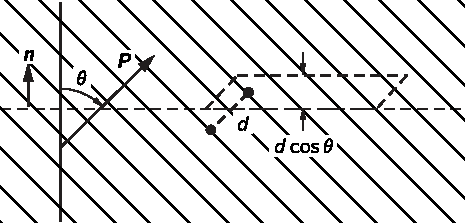
\includegraphics[width=0.9\linewidth]{fyz_fig710.pdf}
      \caption{Náboj, který prošel v dielektriku elementární myšlenou ploškou, je přímo úměrný
               složce vektoru \(\vec{P}\) ve směru normály k ploše. (\cite[s.~179]{Feynman02})}
      \label{fyz:fig710}
    \end{figure}

    Zabývejme se nyní něčím trochu složitějším - případem, kdy elektrická polarizace \(\vec{P}\)
    není všude stejná. Jak jsme již řekli, není-li polarizace konstantní, je možné obecně očekávat
    nenulovou objemovou hustotu náboje, protože z jedné strany může do malého objemového elementu
    vejít více náboje, než z něj může na druhé straně vyjít. Jak zjistíme, kolik náboje do malého
    objemu přibylo nebo se z něj ztratilo? Nejdříve vypočtěme, jaký náboj projde myšlenou plochou
    při polarizaci látky. V případě, že polarizace má směr normály k ploše, množství náboje
    procházející plochou je rovno součinu P a obsahu plochy. Samozřejmě, když má polarizace směr
    tečny k ploše, neprochází plochou žádný náboj.

    Týmiž úvahami, které jsme již provedli, se snadno přesvědčíme, že náboj, jenž projde libovolným
    plošným elementem, je přímo úměrný \emph{složce vektoru \(\vec{P}\) kolmé na plochu}. Porovnejme
    obr. \ref{fyz:fig710} s obr. \ref{fyz:fig709}. Vidíme, že vztah (\ref{fyz:eq911}) je nutné
    obecně psát takto:
    \begin{equation}\label{fyz:eq918}
      σ_{\text{pol}}=\vec{P}\cdot\vec{n}.
    \end{equation}

    Máme-li na mysli plošný element uvnitř dielektrika, udává vztah (\ref{fyz:eq918}) náboj, který
    prošel plochou, ale nevede k vzniku plošného náboje, neboť příspěvky od dielektrika jsou po obou
    stranách plochy stejné a mají opačná znaménka.

    \begin{figure}[ht!] %\ref{fyz:fig711}
      \centering
      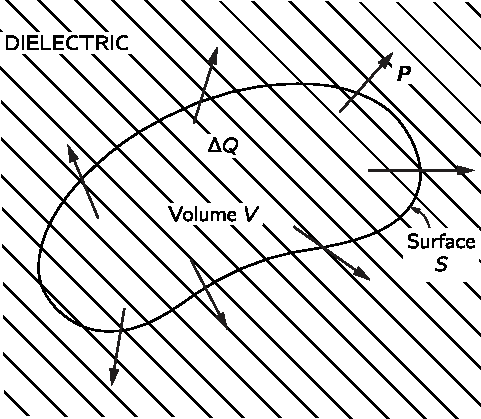
\includegraphics[width=0.9\linewidth]{fyz_fig711.pdf}
      \caption{Nehomogenní polarizace \(\vec{P}\) může vést ke vzniku náboje v objemu dielektrika.
               (\cite[s.~707]{Feynman02})}
      \label{fyz:fig711}
    \end{figure}

    Posunutí nábojů však mohou vést ke vzniku objemové hustoty náboje. Celkový náboj vysunutý
    polarizací ven z néjakého objemu \(V\) je roven integrálu normálové složky vektoru \(\vec{P}\)
    plochou \(S\), která ohraničuje \(V\) (obr. \ref{fyz:fig711}). Stejně velký přebytek náboje
    opačného znaménka zůstane uvnitř. Označíme-li jej \(ΔQ_{\text{pol}}\), bude platit
    \begin{equation}\label{fyz:eq919}
      \Delta Q_{\text{pol}}=-\int_S\vec{P}\cdot\vec{n}\dd{S}.
    \end{equation}
    \(\Delta Q_{\text{pol}}\) můžeme vyjádřit pomocí objemového rozdělení náboje s hustotou
    \(ρ_{\text{pol}}\)
    \begin{equation}\label{fyz:eq920}
      \Delta Q_{\text{pol}}=\int_V\rho_{\text{pol}}\dd{V}.
    \end{equation}
    Z rovnosti pravých stran obou těchto výrazů vyplývá
    \begin{equation}\label{fyz:eq921}
      \int_V\rho_{\text{pol}}\dd{V}=-\int_S\vec{P}\cdot\vec{n}\dd{S}.
    \end{equation}
    Dostali jsme něco jako Gaussovu větu, která uvádí do souvislosti hustotu náboje v polarizovaných
    látkách a vektor elektrické polarizace \(vec{P}\). Můžeme se přesvědčit, že souhlasí s
    výsledkem, který jsme dostali pro povrchový polarizační náboj nebo pro dielektrikum v deskovém
    kondenzátoru. Aplikujeme-li rovnici (\ref{fyz:eq921}) na gaussovskou plochu z obr.
    \ref{fyz:fig705}, bude plošný itegrál roven \(PΔS\) a náboj uvnitř plochy bude
    \(\sigma_{\text{pol}}\,\Delta S\), takže opět dostáváme \(σ_{\text{pol}}=P\).
    
    Stejně jako v případě elektrostatického Gaussova zákona můžeme i rovnici (\ref{fyz:eq921})
    transformovat na diferenciální tvar použitím Gaussovy věty z matematiky:
    \begin{equation*}
      \int_S\vec{P}\cdot\vec{n}\dd{S}=\int_V∇\cdot\vec{P}\dd{V}.
    \end{equation*}
    Dostaneme
    \begin{equation}\label{fyz:eq922}
      ρ_{\text{pol}}=−∇⋅\vec{P}.
    \end{equation}
    Je-li polarizace nehomogenní, dává její divergence výslednou hustotu náboje vznikající v látce.
    Zdůrazňujeme, že jde o naprosto \emph{reálnou} hustotu náboje; „polarizačním nábojem“ jej
    nazýváme proto, abychom připomněli, odkud se vzal.

  \section{Elektrostatické rovnice pro dielektrika}\label{fyz:IIchapXsecIV}
    Nyní už spojme uvedený výsledek s naší elektrostatickou teorií. Základní rovnice je
    \begin{equation}\label{fyz:eq936}
      ∇\cdot\vec{E}=\dfrac{\varrho}{\varepsilon_0}.
    \end{equation}
    kde \(ρ\) je hustota všech elektrických nábojů. Protože není snadné sledovat polarizační náboje,
    je vhodné rozdělit \(ρ\) na dvě části. Opět budeme jako \(ρ_{\text{pol}}\), označovat náboje
    vyvolané nehomogenní polarizací a jako \(ρ_{\text{free}}\) všechny ostatní náboje. Obvykle
    představuje \(ρ_{\text{free}}\) náboj, který jsme přivedli na vodiče, nebo náboj, který je v
    prostoru rozdělen známým způsobem. Rovnice (\ref{fyz:eq923}) pak získá tvar
    \begin{equation*}
      ∇⋅\vec{E}=\dfrac{ρ_{\text{free}}+ρ_{\text{pol}}}{\varepsilon_0}
               =\dfrac{ρ_{\text{free}}−∇⋅\vec{P}}{\varepsilon_0}
    \end{equation*}
    resp. 
    \begin{equation}\label{fyz:eq923}
      ∇\cdot\left(\vec{E}+\dfrac{\vec{P}}{\varepsilon_0}\right)
        =\dfrac{ρ_{\text{free}}}{\varepsilon_0}.
    \end{equation}
    Rovnice pro \(\rot{E}\) se, přirozeně, nemění, tj.
    \begin{equation}\label{fyz:eq924}
      ∇×\vec{E}=0.
    \end{equation}

    Dosadíme-li \(\vec{P}\) ze vztahu (\ref{fyz:eq914}), dostaneme jednodušší rovnici
    \begin{equation}\label{fyz:eq925}
      ∇\cdot[(1+χ)\vec{E}]=∇⋅(\varepsilon_0\vec{E})=\dfrac{ρ_{\text{free}}}{\varepsilon_0}.
    \end{equation}
    To jsou rovnice elektrostatiky pro dielektrika. Přirozeně, neříkají nic nového, jsou pouze v
    takovém tvaru, který je vhodnější pro výpočet v případech, kdy \(ρ_{\text{free}}\) je známé a
    vektor polarizace \(\vec{P}\) je přímo úměrný poli \(\vec{E}\).

    Všimněme si, že relativní permitivitu \(\varepsilon_r\) jsme nevytkli před symbol divergence. Je
    to proto, že nemusí být všude stejná. Má-li všude stejnou hodnotu, může být vytknuta jako
    součinitel a naše rovnice budou přesně takové, jaké jsme měli v elektrostatice, pouze hustota
    náboje bude vydělena hodnotou \(\varepsilon_r\). Ve tvaru, ve kterém jsme je uvedli, se hodí pro
    obecný případ, kdy se na různých místech v poli mohou nacházet různá dielektrika. Může se však
    stát, že tyto rovnice potom budou jen obtížně řešitelné.

    Je třeba se zde zmínit o jedné okolnosti důležité z historického hlediska. V prvním období nauky
    o elektřině nebyl znám atomový mechanizmus polarizace a o existenci \(ρ_{\text{free}}\) se
    nevědělo. Náboj \(ρ_{\text{free}}\) byl pokládán za celkovou hustotu nábojů. Aby se Maxwellovy
    rovnice mohly psát v jednoduchém tvaru, byl definován nový vektor \(\vec{D}\) rovnající se
    lineární kombinaci vektorů \(\vec{E}\) a \(\vec{P}\).
    \begin{equation}\label{fyz:eq926}
      \vec{D}=\varepsilon_0\vec{E}+\vec{P}.
    \end{equation}
    V důsledku toho se rovnice (\ref{fyz:eq923}) a (\ref{fyz:eq924}) psaly ve zdánlivě jednoduchém
    tvaru:
    \begin{equation}\label{fyz:eq927}
      ∇\cdot\vec{D}=ρ_{\text{free}},\qquad ∇×\vec{E}=0.
    \end{equation}
    Lze je řešit? Pouze je-li udána i třetí rovnice, vyjadřující vztah mezi \(\vec{D}\) a
    \(\vec{E}\). Platí-li (\ref{fyz:eq923}), je tento vztah
    \begin{equation}\label{fyz:eq928}
      \vec{D}=\varepsilon_0(1+χ)\vec{E}=\varepsilon_r\varepsilon_0\vec{E}.
    \end{equation}
    Tato rovnice byla obvykle psána ve tvaru
    \begin{equation}\label{fyz:eq929}
      \vec{D}=\varepsilon\vec{E},
    \end{equation}
    kde \(\varepsilon\) představuje další konstantu popisující elektrické vlastnosti látek. Nazývá
    se \textbf{permitivita}. (Nyní vidíme, proč v našich rovnicích vystupuje \(\varepsilon_0\) -
    jako permitivita vakua). Zřejmě
    \begin{equation}\label{fyz:eq930}
      \varepsilon=\varepsilon_r\varepsilon_0=(1+χ)\varepsilon_0.
    \end{equation}
    
    Dnes se na tyto záležitosti díváme z jiného hlediska. Pro vakuum totiž bereme jednodušší
    rovnice, a započteme-li v každém případě všechny náboje bez ohledu na jejich původ, budou tyto
    rovnice platit vždy. Oddělíme-li některé z nábojů ať už pro pohodlnost nebo proto, že nehodláme
    detailně zkoumat, co se děje, můžeme, chceme-li, psát naše rovnice v jakémkoliv jiném tvaru.

    Ještě jednu věc je třeba zdůraznit. Rovnice typu \(\vec{D}=\varepsilon_0\vec{E}\) představuje
    pokus popsat vlastnosti látky. Ale látka je krajně složitá a takováto rovnice ve skutečnosti
    není správná. Například, bude-li \(\vec{E}\) příliš velké, přestane být \(\vec{D}\) přímo úměrné
    \(\vec{E}\). Pro některé látky přestává přímá úměrnost už při poměrně malých polích. Kromě toho
    „konstanta“ úměrnosti může záviset na tom jak rychle se \(\vec{E}\) mění v čase. Proto rovnice
    takového typu představuje jakousi aproximaci podobně jako Hookův zákon. Nemůže to být hluboká a
    fundamentální rovnice. Naproti tomu naše základní rovnice pro \(\vec{E}\) (\ref{fyz:eq923}) a
    (\ref{fyz:eq924}) vyjadřují naše nejhlubší a nejúplnější pochopení elektrostatiky.
    
  \section{Pole a síly v přítomnosti dielektrik}\label{fyz:IIchapXsecV}       
    Nyní dokážeme některé dost obecné věty elektrostatiky pro takové situace, v nichž se vyskytují i
    dielektrika. Viděli jsme, že když se prostor mezi elektrodami deskového kondenzátoru vyplní
    dielektrikem, kapacita kondenzátoru se v určitém poměru zvětší. Lze ukázat, že to platí pro
    kondenzátor \emph{každého} tvaru za předpokladu, že celý prostor v okolí obou vodičů je vyplněn
    homogenním lineárním dielektrikem. V případě bez dielektrika je třeba řešit tyto rovnice
    \begin{align}
      ∇\cdot\vec{E}_0             &=\dfrac{ρ_{\text{free}}}{\varepsilon_0}, \quad
      ∇\times\vec{E}_0=0. \label{fyz:eq931} \\
      \shortintertext{V přítomnosti dielektrika se první z těchto rovnic změní, a budeme tedy mít 
      rovnice}
      ∇\cdot(\varepsilon_r\vec{E})&=\dfrac{ρ_{\text{free}}}{\varepsilon_0}, \quad
      ∇\times\vec{E}=0.  \label{fyz:eq932}   \\
      \shortintertext{Protože \(\varepsilon_r\) považujeme všude za stejné, je možné je zapsat
      takto:}
      ∇\cdot(\varepsilon_r\vec{E})&=\dfrac{ρ_{\text{free}}}{\varepsilon_0}, \quad 
      ∇\times(\varepsilon_r\vec{E})=0.  \label{fyz:eq933}
    \end{align}

    Pro veličinu \(\varepsilon_r\vec{E}\) máme proto stejné rovnice jako pro \(\vec{E}_0\), jejich
    řešením je tedy \(\varepsilon_r\vec{E}=\vec{E}_0\). Jinými slovy, pole bude všude slabší v
    poměru \(1/\varepsilon_r\) vzhledem k tomu, jaké by bylo bez dielektrika. Jelikož rozdíl
    potenciálů je křivkovým integrálem intenzity pole, v tomtéž poměru se zmenší i napětí. Protože
    náboj na elektrodách kondenzátoru se bral v obou případech stejný, ze vztahu (\ref{fyz:eq908})
    vyplývá, že kapacita kondenzátoru se všude homogenním dielektrikem vzroste
    \(\varepsilon_r\)-krát.

    Nyní se zeptejme, jaká síla působí mezi dvěma nabitými vodiči v dielektriku. Uvažujme tekuté
    dielektrikum, které je všude homogenní. Už jsme viděli, že jeden způsob, jak dostat sílu, je
    derivovat energii podle vhodné vzdálenosti. Mají-li vodiče stejně velké opačné náboje, je
    energie \(W= q^2/2C\), kde \(C\) je jejich kapacita. Podle principu virtuální práce je každá
    složka síly dána derivací, například
    \begin{equation}\label{fyz:eq934}
      F_x=-\diffp{U}{x}=-\frac{Q^2}{2}\diffp{}{x}\left(\dfrac{1}{C}\right).
    \end{equation}
    Protože dielektrikum zvětšuje kapacitu \(\varepsilon_r\)-krát, musíme všechny síly
    \emph{zmenšit} ve stejném poměru.

    Je třeba zdůraznit jednu věc. Co jsme řekli platí pouze tehdy, když je dielektrikum tekutina.
    Každý pohyb vodičů zapuštěných v pevném dielektriku mění podmínky pro vznik mechanických napětí
    v dielektriku, jeho elektrické vlastnosti a vyvolává i změnu mechanické energie dielektrika.
    Pohyb vodičů v tekutině nemění tekutinu. Tekutina se sice přemístí na nové místo, ale její
    elektrické charakteristiky se nezmění.
      
    Mnohé starší knihy o elektřině vycházejí ze „základního“ zákona, že síla působící mezi dvěma
    náboji je
    \begin{equation}\label{fyz:eq935}
      F=\dfrac{q_1q_2}{4\pi\varepsilon_0\varepsilon_r r^2},
    \end{equation}
    Toto hledisko je naprosto neuspokojivé. Zaprvé, tento zákon neplatí obecně; platí pouze ve světě
    zaplněném tekutinou. Za druhé, závisí na skutečnosti, že \(\varepsilon_r\) je konstanta, což pro
    většinu reálných látek platí pouze přibližně. Je mnohem lepší začít Coulombovým zákonem pro
    náboje ve vakuu, který je správný vždy (pro nepohybující se náboje).

    Co se stane v pevné látce? To je velmi obtížný problém, který není vyřešen, neboť je v určitém
    smyslu neurčitý. Vkládáme-li náboje dovnitř pevného dielektrika, vznikají mnohé tlaky a napětí.
    Nemůžete tedy pracovat s virtuální prací, aniž bychom zahrnuli i mechanickou energii potřebnou
    na stlačení pevné látky. Obecně je však těžké jednoznačně rozlišit elektrické síly od
    mechanických sil vyvolaných samotnou pevnou látkou. Naštěstí, ve skutečnosti nikdo nikdy
    nepotřebuje znát odpověď na námi položenou otázku. Někdy je snad třeba znát velikost napětí
    vznikajících v pevné látce a to lze spočítat. Je to však mnohem složitější než jednoduchý
    výsledek, který jsme dostali pro tekutiny.

    V teorii dielektrik je překvapivě složitý následující problém: Proč nabité těleso přitahuje malé
    kousky dielektrika? Když si v suchý den pročešeme vlasy, hřeben ihned přitáhne malé útržky
    papíru. Pokud jsme o tom přemýšleli povrchně, pravděpodobně nás napadlo, že na hřebeni je náboj
    jednoho druhu, zatímco papír má náboj opačný. Ale papír byl původně elektricky neutrální. Nemá
    žádný zbytkový náboj, ale i tak je přitahován. Je pravda, že někdy papírek přiskočí k hřebenu a
    potom odskočí, odpuzen okamžitě, jakmile se hřebene dotkl. Příčina je, samozřejmě, v tom, že
    když se papírek dotkne hřebene, přibere nějaké záporné náboje a stejné náboje se pak odpuzují.
    Ale to není odpověď na původní otázku. Proč papírek přiskočí k hřebeni poprvé?

    \begin{figure}[ht!] %\ref{fyz:fig712}
      \centering
      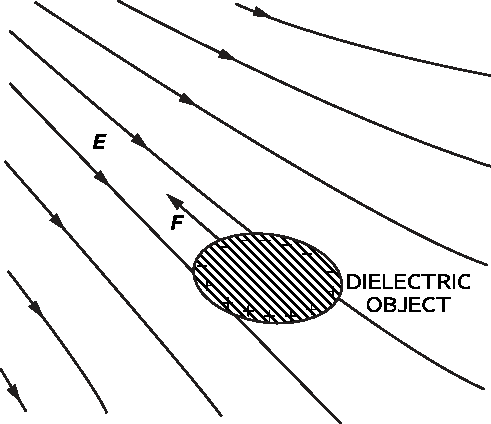
\includegraphics[width=0.8\linewidth]{fyz_fig712.pdf}
      \caption{V nehomogenním poli působí na dielektrické těleso síla směřující do prostoru s vyšší
              intenzitou pole. (\cite[s.~184]{Feynman02})}
      \label{fyz:fig712}
    \end{figure}

    Můžeme to vysvětlit polarizací dielektrika, nacházejícího se v elektrickém poli. Vznikají
    polarizační náboje obou znamének, které jsou hřebenem přitahovány, resp. odpuzovány. Výsledkem
    však bude přitahování, protože blíže k hřebenu je pole silnější než dál od něj - hřeben není
    nekonečnou rovinou. Jeho náboj je lokalizovaný. Neutrální kousíček papíru se nepřitáhne ani k
    jedné z elektrod rovinného kondenzátoru. Nehomogenita pole představuje podstatnou část
    mechanizmu přitahování.

    Jak ukazuje obr. \ref{fyz:fig712}, je dielektrikum vždy přitahováno z oblasti se slabým polem do
    oblasti se silnějším polem. Je možné dokázat, že pro malá tělesa je síla přímo úměrná gradientu
    druhé mocniny intenzity elektrického pole. Proč závisí na druhé mocnině intenzity pole? Protože
    indukované polarizační náboje jsou přímo úměrné polím a pro dané náboje jsou síly přímo úměrné
    poli. Ale jak jsme právě naznačili, bude výsledná síla nenulová pouze tehdy, když se druhá
    mocnina pole od bodu k bodu mění. Součinitel úměrnosti obsahuje mezi jiným permitivitu tělesa a
    závisí i na velikosti a tvaru tělesa.

    \begin{figure}[ht!] %\ref{fyz:fig713}
      \centering
      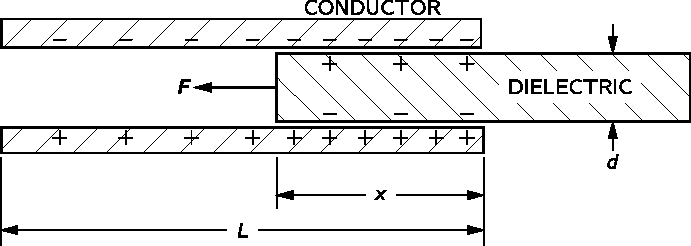
\includegraphics[width=0.9\linewidth]{fyz_fig713.pdf}
      \caption{Sílu působící v deskovém kondenzátoru na dielektrickou destičku můžeme vypočítat
               použitím principu zachování energie. (\cite[s.~707]{Feynman02})}
      \label{fyz:fig713}
    \end{figure}

    Existuje příbuzná úloha, v níž je možné vypočítat sílu působící na dielektrikum zcela přesně.
    Máme-li deskový kondenzátor s dielektrickou destičkou vsunutou mezi elektrody pouze částečně
    {obr. \ref{fyz:fig713}), vznikne síla vtahující dielektrikum dovnitř. Podrobné prozkoumání této
    síly je velmi složité; souvisí s nehomogenitami pole v blízkosti hran dielektrika a elektrod.
    Ale odhlédneme-li od téchto detailů a použijeme pouze princip zachování energie, můžeme sílu
    jednoduše vypočítat. Najdeme ji ze vzorce, který jsme už odvodili dříve. Vztah (\ref{fyz:eq934})
    je ekvivalentní se vztahem
    \begin{equation}\label{fyz:eq937}
      F_x=-\diffp{U}{x}=-\frac{Q^2}{2}\diffp{}{x}\left(\frac{1}{C}\right).
    \end{equation}
    Potřebujeme pouze zjistit, jak se kapacita méní v závislosti na poloze dielektrické destičky.

    Předpokládejme, že celková délka elektrod je \(L\), jejich šířka je \(w\), jejich vzájemná
    vzdálenost, jakož i tloušťka dielektrika je \(d\) a vzdálenost, do které bylo dielektrikum
    zasunuto, je \(x\). Kapacita představuje poměr celkového volného náboje na elektrodách k napětí
    mezi nimi. Viděli jsme, že pro dané napětí \(U\) je plošná hustota volného náboje
    \(\varepsilon_r\varepsilon_0U/d\). Celkový náboj na elektrodách tedy je
    \begin{equation*}
      Q=\frac{\varepsilon_r\varepsilon_OU}{d}xW+\dfrac{\varepsilon_O U}{d}(L-x)W,
    \end{equation*}

  \section{Příklady a cvičení}\label{fyz:IIchapXsecVI}



\todo[inline]{Kapitola fey2ch10 je nedodělaná, obsahuje pouze obrázky}
%} %tikzset
%---------------------------------------------------------------------------------------------------
